\chapter{Ergebnisse}

\section{Präzision und Inferenzverhalten}

\subsection*{SSD}

Ursprünglich wurden 500 Epochen für das Training vorgesehen für jeden der Kreuzvalidierungsschritte. Da allerdings beim Training schon nach knapp über hundert Epochen sich der Gradient der Kostenfunktion nur träge veränderte, wurde im Sinne des \textit{Early Stoppings} nach 120 Epochen das Training vorzeitig beendet, um \textit{Overfitting} zu vermeiden. Das niedrigste Ergebnis der Kostenfunktion betrug 1.726. Es ergab eine \textit{mAP} von 83.1\%, leicht über den Referenzergebnissen von \textit{SSD} zu \textit{PascalVOC} (siehe Abbildung \ref{result}). Die Ergebnisse zu den einzelnen Klassen sind in folgender Tabelle dargestellt:

\begin{center}
	\begin{tabular}[h]{l|c}
		Klasse & mAP \\
		\hline
		Saskia Wasser Groß & 77.62\% \\
		Saskia Wasser Klein & 75.96\% \\
		Pepsi Cola Groß & 94.94\% \\
		Pepsi Cola Klein & 86.38\% \\
		ISO & 86.37\% \\
		ACE & 85.43\% \\
		Stenger Johannisbeerschorle & 69.47\% \\
		Stenger Apfelsaftschorle & 82.48 \% \\
		Vitamalz Malzbier & 76.24\%
	\end{tabular}
	\captionof{table}{Validierungsergebnisse SSD}
	\label{table:ssdresults}
\end{center}

Wird nun das trainierte Modell auf echte Daten angewendet, so fällt auf, dass manche Objekte doppelt detektiert werden. Um dieses Problem zu lösen, gibt es zwei Möglichkeiten. 

Als erstes kann bei der Detektion der minimale \textit{confidence score} angegeben werden, ab wann eine Detektion offiziell als solche wahrgenommen wird. Hier liegt die Herausforderung darin, einen optimalen Wert zu finden, sodass verdeckte Objekte noch als solche erkannt werden, aber doppelt erkannte Objekte nicht mehr auftreten. Der \textit{confidence score} wurde nach mehrmaligem Iterieren auf 0.75 festgelegt.

Die zweite Möglichkeit besteht darin, die maximale Überlappung zweier Bounding Boxen festzulegen. Somit werden doppelte Bounding Boxen, die sich flächenmäßig über einem gewissen Grenzwert überlappen, auf eine Bounding Box reduziert. Er stellte ich sich Parameter von 0.5 als geeignet heraus.

Außerdem wurden Inkonsistenzen im Detektionsverhalten festgestellt:

\begin{figure}[ht]
	\centering
	\subfigure[verdeckt]{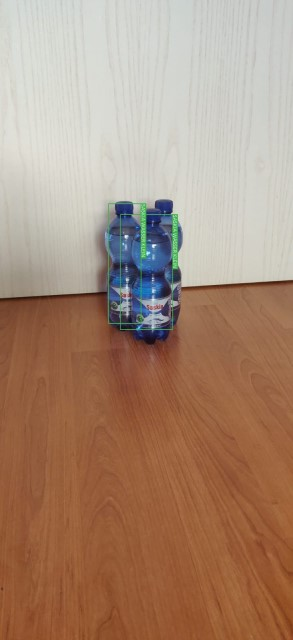
\includegraphics[width=0.30\textwidth]{Bilder/verdeckt.jpeg}}
	\hspace{2cm}
	\subfigure[winkel]{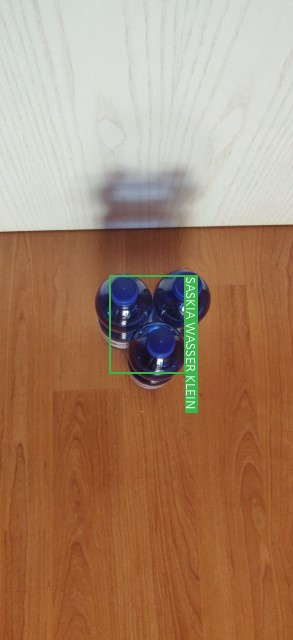
\includegraphics[width=0.30\textwidth]{Bilder/winkel.jpeg}}
	\caption{Detektionsverhalten bei extremen Blicklagen}
	\label{lagen}
\end{figure}

So sind von anderen Objekten verdeckte Objekte nur schwer zu erkennen, genauso wie Objekte aus extremen Blicklagen (siehe Abbildung \ref{lagen}). Diese Fälle wurden im Datensatz zwar zu 12.5\% abgedeckt, es lässt sich aber keine Aussage darüber treffen, ob eine Erweiterung des Datensatzes eine Abhilfe für dieses Problem hätte liefern können. 

\begin{figure}[ht]
	\subfigure[1 Meter]{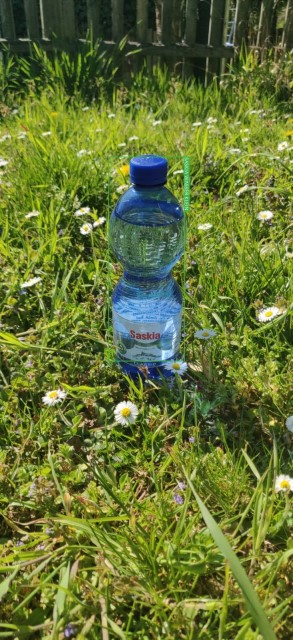
\includegraphics[width=0.30\textwidth]{Bilder/einmeter.jpeg}}\hfill
	\subfigure[2 Meter]{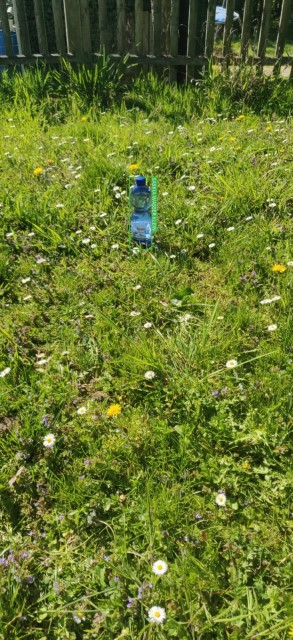
\includegraphics[width=0.30\textwidth]{Bilder/zweimeter.jpeg}}\hfill
	\subfigure[3 Meter]{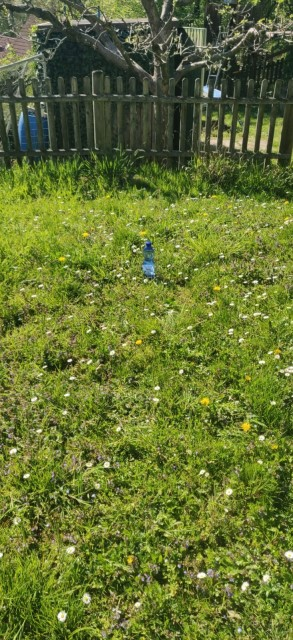
\includegraphics[width=0.30\textwidth]{Bilder/dreimeter.jpeg}}\hfill
	\caption{Detektionsverhalten bei unterschiedlichen Entfernungen}
	\label{entfernung}
\end{figure}

Auch die Entfernung zum zu detektierenden Objekt besitzt eine Auswirkung auf das Detektionsverhalten. In Abbildung \ref{entfernung} wird gezeigt, dass ab einer Entfernung von drei Metern keine Detektion mehr erfolgte. 

\begin{figure}[ht]
	\subfigure[überbeleuchtet]{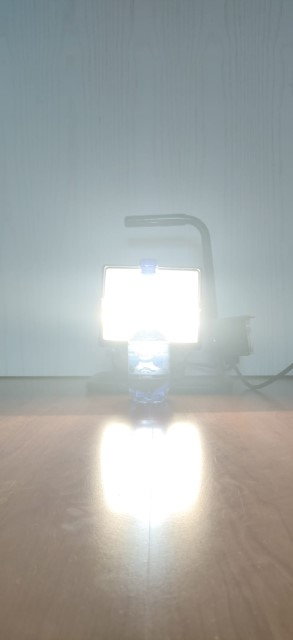
\includegraphics[width=0.30\textwidth]{Bilder/ueberbeleuchtet.jpeg}}\hfill
	\subfigure[normal]{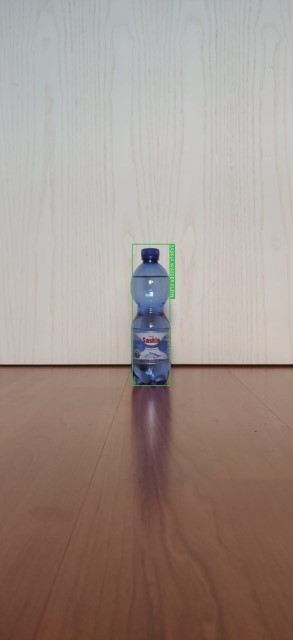
\includegraphics[width=0.30\textwidth]{Bilder/normalbeleuchtet.jpeg}}\hfill
	\subfigure[unterbeleuchtet]{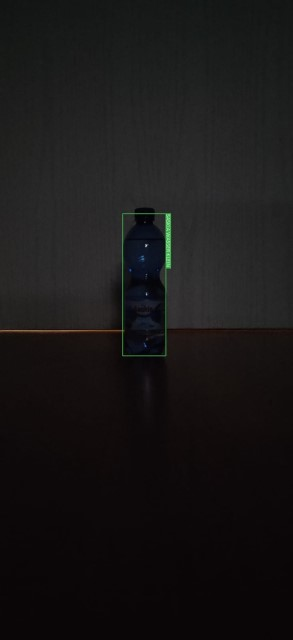
\includegraphics[width=0.30\textwidth]{Bilder/unterbeleuchtet.jpeg}}\hfill
	\caption{Detektionsverhalten bei unterschiedlichen Beleuchtungsverhältnissen}
	\label{sicht}
\end{figure}

Des Weiteren haben unterschiedliche Beleuchtungsgrade eine Auswirkung auf das Detektionsverhalten. In Abbildung \ref{sicht} wird unterschieden zwischen dem Detektionsverhalten bei überbeleuchteten, normalen und unterbeleuchteten Sichtverhältnissen. Überbeleuchtete Umgebungsverhältnisse erschweren die Objektdetektion in diesem Beispiel. 

Die Detektion reagierte allerdings invariant gegenüber unterschiedlichen Hintergründen oder Bildauflösungen.

\subsection*{YOLO}

Um eine möglichst gute Aussage über den Vergleich der beiden Objektdetektoren treffen zu können kommt bei \textit{YOLO} der exakt gleiche Trainings- und Testdatensatz wie beim \textit{SSD} zum Einsatz. Das Training von \textit{YOLO} ergab eine \textit{mAP} von 80.36\%. Abbildung \ref{yolo_result} zeigt die Verbesserung des Modells während dem Trainingsprozess. 

\begin{figure}[H]
	\begin{center}
		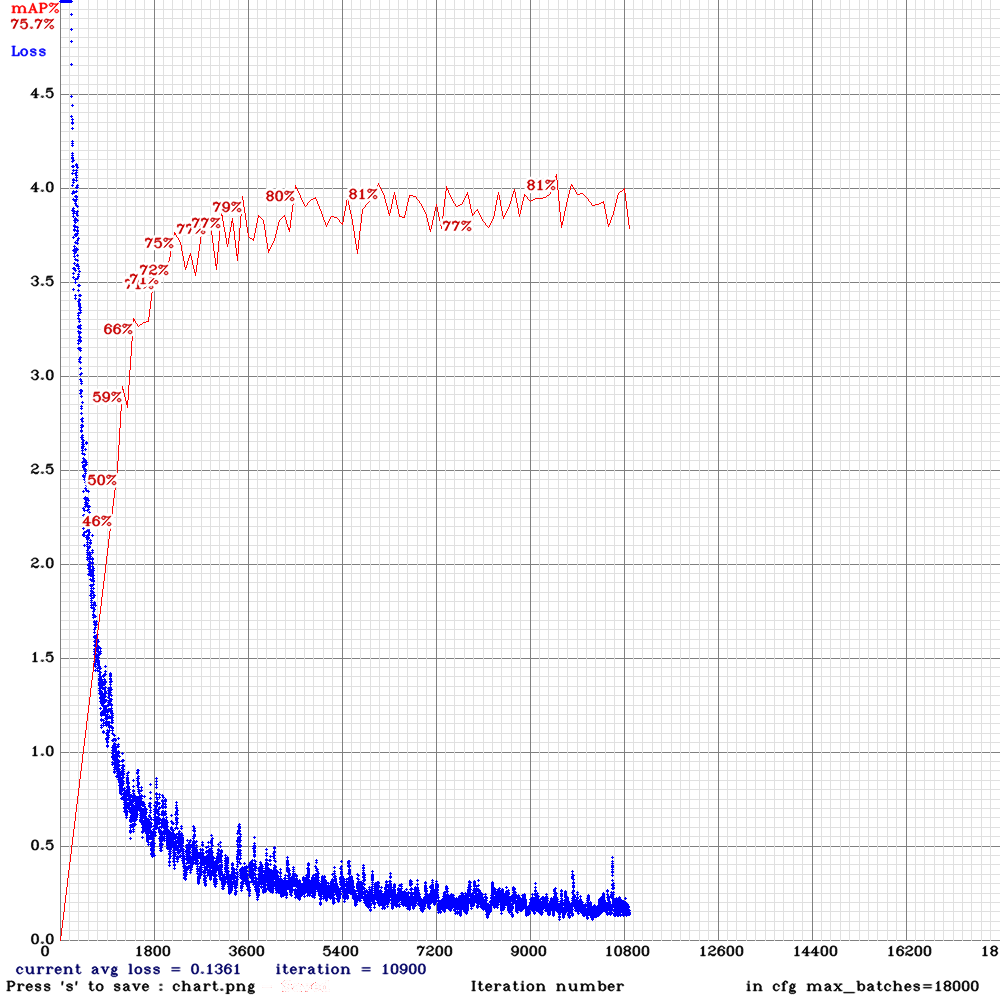
\includegraphics[width=13cm]{Bilder/yolo_result.png} 
		\caption{\textit{YOLO}: Entwicklung von durchschnittlichem Verlust (avg loss) und \textit{mAP} während dem Training}
		\label{yolo_result}
	\end{center}
\end{figure}

Wie beim \textit{SSD} erreicht das Modell relativ frühzeitig nach bereits etwa 3600 Batches eine \textit{mAP} von 79\%. Das Training wurde daher vor Erreichung der durch die Dokumentation nahegelegte maximale Anzahl an Batches nach 11000 Batches abgebrochen. Das kann darauf zurückgeführt werden, dass es sich bei den gelabelten Klassen um Objekte des gleichen Typs handelt und das Modell dementsprechend leichter trainiert werden kann. 

Der \textit{confidence score} liegt standardmäßig bei 0.25. Nach mehreren Durchläufen stellt sich heraus, dass dieser Wert nicht verändert werden sollte. Ein zu geringer Wert sorgt zwar dafür, dass möglicherweise mehr Objekte erkannt werden. Allerdings steigt damit auch die Rate an falsch oder doppelt erkannter Objekte. Ein Parameter für die Obergrenze der Überlappung zweier Bounding Boxen existiert nicht.

Tabelle \ref{table:yoloresults} zeigt die \textit{mAP} für jede gelabelte Klasse:

\begin{center}
	\begin{tabular}[H]{l|c}
		Klasse & mAP \\
		\hline
		Saskia Wasser Groß & 76.69\% (-0.93\%)\\
		Saskia Wasser Klein & 80.63\% (+4.67\%)\\
		Pepsi Cola Groß & 73.14\% (-21.8\%)\\
		Pepsi Cola Klein & 75.24\% (-11.14\%)\\
		ISO & 90.28\% (+3.91\%)\\
		ACE & 86.69\% (+1.26\%)\\
		Stenger Johannisbeerschorle & 72.50\% (+3.03\%)\\
		Stenger Apfelsaftschorle & 78.05\% (-4.43\%)\\
		Vitamalz Malzbier & 81.94\% (+5.7\%)
	\end{tabular}
	\captionof{table}{Validierungsergebnisse YOLO mit Vergleich zu \textit{SSD}}
	\label{table:yoloresults}
\end{center}

Auffällig niedrig ist die \textit{mAP} der Klassen \textit{Pepsi Cola Groß} und \textit{Pepsi Cola Klein}. Ein Wertevergleich gibt jedoch keinen guten Einblick in den Unterschied der zwei trainierten Modelle in der Praxis. Im folgenden wird daher das Detektionsverhalten auf den gleichen Bildern wie zuvor beim \textit{SSD} evaluiert:

\begin{figure}[H]
	\centering
	\subfigure[verdeckt]{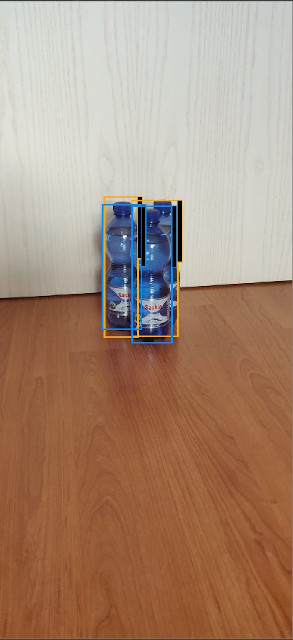
\includegraphics[width=0.30\textwidth]{Bilder/yolo_verdeckt.jpg}}
	\hspace{2cm}
	\subfigure[winkel]{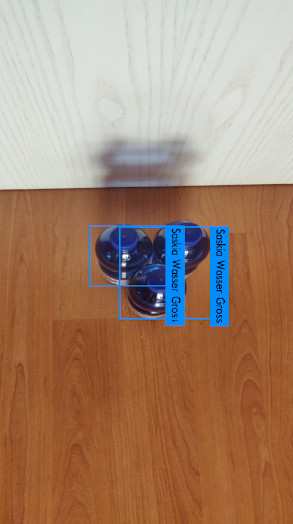
\includegraphics[width=0.30\textwidth]{Bilder/yolo_winkel.jpg}}
	\caption{Detektionsverhalten von \textit{YOLO} bei extremen Blicklagen}
	\label{lagen_yolo}
\end{figure}

Auch bei \textit{YOLO} können verdeckte Objekte nur schwer erkannt werden. Ein Unterschied zeigt sich bei der Ansicht von oben (siehe Abbildung \ref{lagen_yolo}). Hier werden zwei von drei Flaschen erkannt, die allerdings der falschen Klasse (\textit{Saskia Wasser Groß} statt \textit{Saskia Wasser Klein}) zugeordnet werden und eine der zwei Bounding Boxes zwei Flaschen umschließt.

\begin{figure}[H]
	\subfigure[1 Meter]{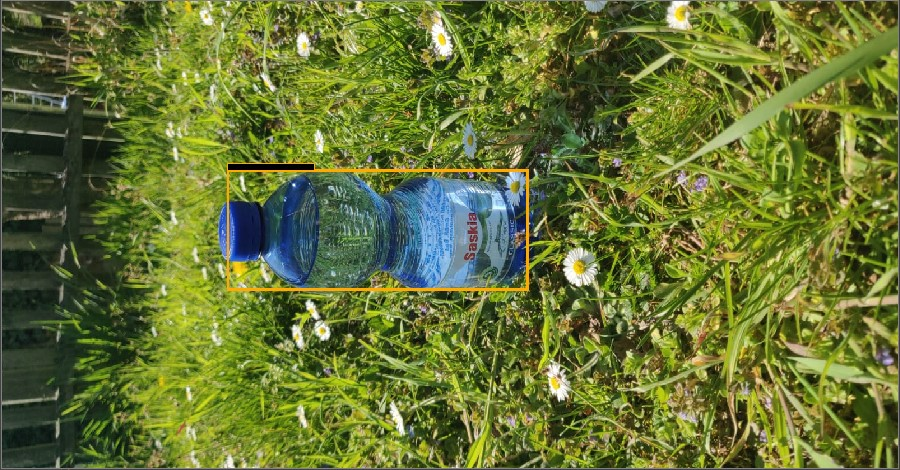
\includegraphics[width=0.30\textwidth]{Bilder/yolo_entfernung1.jpg}}\hfill
	\subfigure[2 Meter]{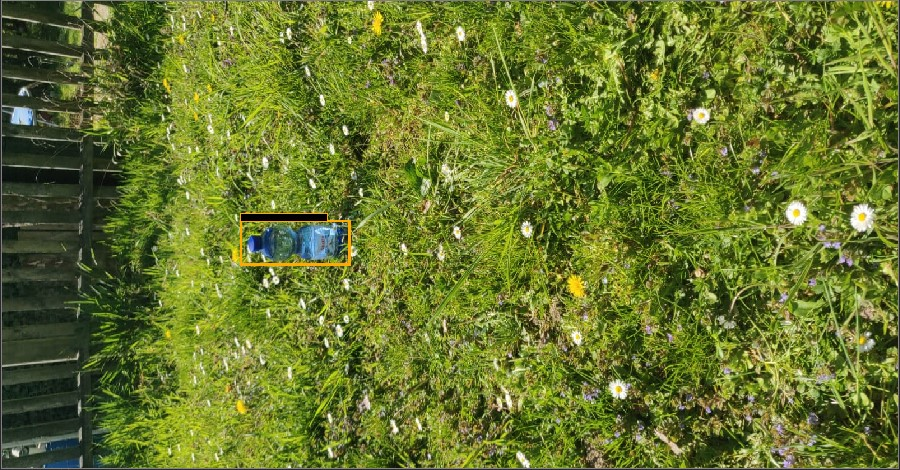
\includegraphics[width=0.30\textwidth]{Bilder/yolo_entfernung2.jpg}}\hfill
	\subfigure[3 Meter]{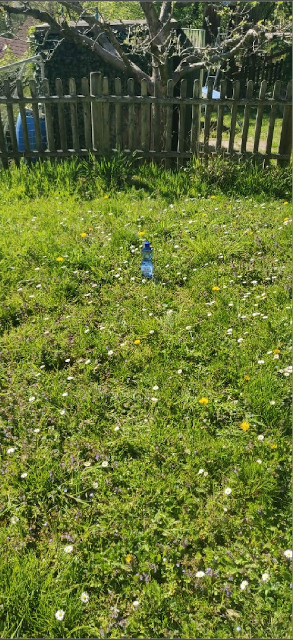
\includegraphics[width=0.30\textwidth]{Bilder/yolo_entfernung3.jpg}}\hfill
	\caption{Detektionsverhalten von \textit{YOLO} bei unterschiedlichen Entfernungen}
	\label{entfernung_yolo}
\end{figure}

Wie bei \textit{SSD} erfolgt nach bereits drei Metern Entfernung keine Detektion mehr (siehe Abbildung \ref{entfernung_yolo}). Der \textit{confidence score} für die korrekt erkannte Bounding Box liegt bei nur 2\%. Beide Modelle sind damit für große Distanzen zwischen der Drohne und den Objekten ungeeignet.
 
\begin{figure}[H]
 	\subfigure[überbeleuchtet]{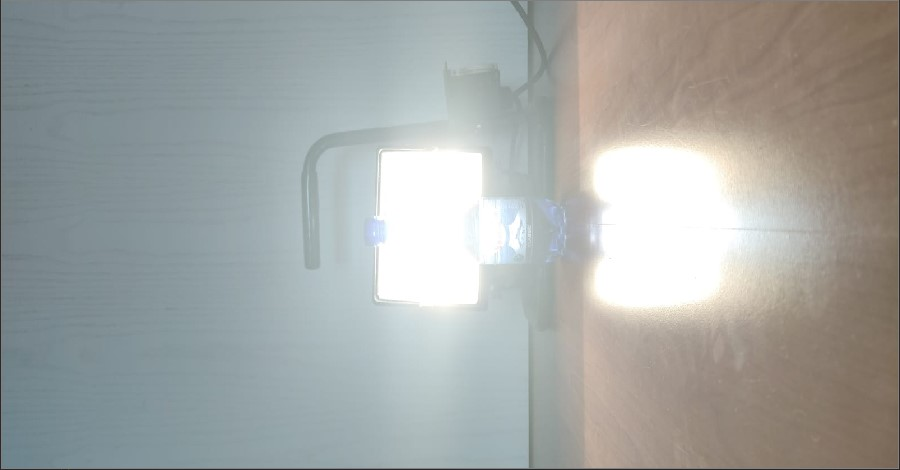
\includegraphics[width=0.30\textwidth]{Bilder/yolo_beleuchtung2.jpg}}\hfill
 	\subfigure[normal]{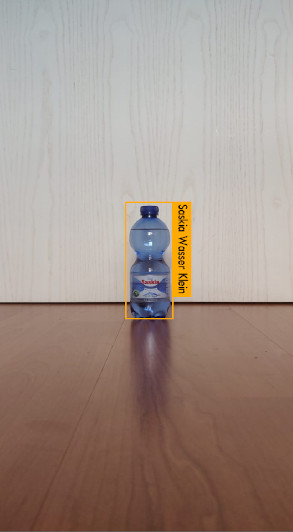
\includegraphics[width=0.30\textwidth]{Bilder/yolo_beleuchtung1.jpg}}\hfill
 	\subfigure[unterbeleuchtet]{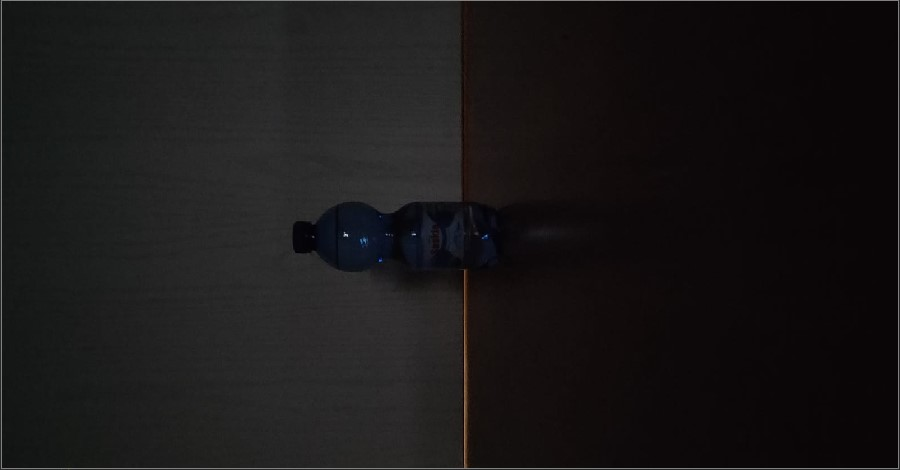
\includegraphics[width=0.30\textwidth]{Bilder/yolo_beleuchtung3.jpg}}\hfill
 	\caption{Detektionsverhalten von \textit{YOLO} bei unterschiedlichen Beleuchtungsverhältnissen}
 	\label{sicht_yolo}
\end{figure}

Beim Testen der verschiedenen Beleuchtungsverhältnisse fällt auf, dass im Gegensatz zum \textit{SSD} die Flasche in der unterbelichteten Umgebung nicht erkannt wird beziehungsweise mit einem \textit{confidence score} von nur 6\%. 
 
\section{Reaktionsvermögen}

Bei der Inferenz fällt allerdings entgegen der Erwartungen auf, dass die Inferenz überdurchschnittlich langsam verläuft. Das Problem lässt sich auf die synchrone Arbeitsweise der bisherigen Detektionsalgorithmen zurück führen, bei dem erst ein neuer Frame des Videostreams angefragt wird, sobald das aktuelle Bild durch die Vorverarbeitung gelaufen ist und durch das Modell inferiert wurde. 

Um dem entgegen zu wirken, wurde ein Bufferkonzept in einem parallelem Thread realisiert, der einzelne Frames zeitgleich zur Inferenz anfragt und zwischenspeichert. Ist der Buffer voll, so werden nach dem \textit{First In First Out} Verfahren die älteren Frames verworfen. Dadurch konnte die FPS Anzahl von \textit{SSD} von maximal 18 auf die vollen 30 und bei \textit{YOLO} von 20 auf 28 gesteigert werden. Dadurch sollten sämtliche Änderungen in der Umgebung rechtzeitig vom Objektdetektor erkannt werden. 

Ein weiteres Problem beschreibt die initiale Latenz zwischen der Inferenz und der Bildaufnahme. Die Inferenz kann erst gestartet werden, sobald die Gewichtungen des Modells initialisiert und geladen wurden. Bei \textit{YOLO} benötigt die Initialisierung etwa drei Sekunden. Das lässt sich umgehen, indem entweder der Thread zur Bildaufnahme verzögern gestartet wird oder dessen Buffer kleiner gewählt wird.

\section{Trainingsverhalten}

Eine Epoche lokales Training mit anschließendem Testen des Durchlaufs beim \textit{SSD} auf einer \textit{NVIDIA GTX 1080} dauert im Schnitt neun Minuten. Die Messung basiert auf einer Batch Größe von 16 Bildern bei insgesamt 998 Bildern pro Epoche. Insgesamt wurden 16,5 Stunden zum Erstellen eines Modells mit dem \textit{SSD} benötigt. Beim Training von \textit{YOLO} benötigt eine Batch mit einer Größe von 64 etwa eine Minute und 30 Sekunden, bis zur Erreichung des optimalen Modells vergehen etwa acht Stunden. Die Dauer der beiden Trainingsdurchläufe lässt sich allerdings nur schwer vergleichen. Zum einen wird für das Training von \textit{YOLO} wie im vorherigen Kapitel erwähnt eine andere GPU verwendet, deren Tensor Kerne den Trainingsprozess merklich beschleunigen. Zum anderen werden die beiden Objektdetektoren in zwei verschiedenen Frameworks implementiert, wodurch ein anderes Trainingsverhalten von Grund auf gegeben ist und Unterschiede in der Performance auftreten können. Bei beiden Verfahren kann das Training durch die Ablage von sogenannten Modell-Checkpoints zu einem späteren Zeitpunkt fortgeführt werden. Das ist vor allem dann von Vorteil, wenn nachträglich Parameter oder Trainingsdaten angepasst werden und kein kompletter Neustart des Trainings erforderlich ist.


